\PassOptionsToPackage{unicode=true}{hyperref} % options for packages loaded elsewhere
\PassOptionsToPackage{hyphens}{url}
%
\documentclass[]{article}
\usepackage{lmodern}
\usepackage{amssymb,amsmath}
\usepackage{ifxetex,ifluatex}
\usepackage{fixltx2e} % provides \textsubscript
\ifnum 0\ifxetex 1\fi\ifluatex 1\fi=0 % if pdftex
  \usepackage[T1]{fontenc}
  \usepackage[utf8]{inputenc}
  \usepackage{textcomp} % provides euro and other symbols
\else % if luatex or xelatex
  \usepackage{unicode-math}
  \defaultfontfeatures{Ligatures=TeX,Scale=MatchLowercase}
\fi
% use upquote if available, for straight quotes in verbatim environments
\IfFileExists{upquote.sty}{\usepackage{upquote}}{}
% use microtype if available
\IfFileExists{microtype.sty}{%
\usepackage[]{microtype}
\UseMicrotypeSet[protrusion]{basicmath} % disable protrusion for tt fonts
}{}
\IfFileExists{parskip.sty}{%
\usepackage{parskip}
}{% else
\setlength{\parindent}{0pt}
\setlength{\parskip}{6pt plus 2pt minus 1pt}
}
\usepackage{hyperref}
\hypersetup{
            pdftitle={Quantium Virtual Internship - Retail Strategy and Analytics - Task 1},
            pdfborder={0 0 0},
            breaklinks=true}
\urlstyle{same}  % don't use monospace font for urls
\usepackage[margin=1in]{geometry}
\usepackage{color}
\usepackage{fancyvrb}
\newcommand{\VerbBar}{|}
\newcommand{\VERB}{\Verb[commandchars=\\\{\}]}
\DefineVerbatimEnvironment{Highlighting}{Verbatim}{commandchars=\\\{\}}
% Add ',fontsize=\small' for more characters per line
\usepackage{framed}
\definecolor{shadecolor}{RGB}{248,248,248}
\newenvironment{Shaded}{\begin{snugshade}}{\end{snugshade}}
\newcommand{\AlertTok}[1]{\textcolor[rgb]{0.94,0.16,0.16}{#1}}
\newcommand{\AnnotationTok}[1]{\textcolor[rgb]{0.56,0.35,0.01}{\textbf{\textit{#1}}}}
\newcommand{\AttributeTok}[1]{\textcolor[rgb]{0.77,0.63,0.00}{#1}}
\newcommand{\BaseNTok}[1]{\textcolor[rgb]{0.00,0.00,0.81}{#1}}
\newcommand{\BuiltInTok}[1]{#1}
\newcommand{\CharTok}[1]{\textcolor[rgb]{0.31,0.60,0.02}{#1}}
\newcommand{\CommentTok}[1]{\textcolor[rgb]{0.56,0.35,0.01}{\textit{#1}}}
\newcommand{\CommentVarTok}[1]{\textcolor[rgb]{0.56,0.35,0.01}{\textbf{\textit{#1}}}}
\newcommand{\ConstantTok}[1]{\textcolor[rgb]{0.00,0.00,0.00}{#1}}
\newcommand{\ControlFlowTok}[1]{\textcolor[rgb]{0.13,0.29,0.53}{\textbf{#1}}}
\newcommand{\DataTypeTok}[1]{\textcolor[rgb]{0.13,0.29,0.53}{#1}}
\newcommand{\DecValTok}[1]{\textcolor[rgb]{0.00,0.00,0.81}{#1}}
\newcommand{\DocumentationTok}[1]{\textcolor[rgb]{0.56,0.35,0.01}{\textbf{\textit{#1}}}}
\newcommand{\ErrorTok}[1]{\textcolor[rgb]{0.64,0.00,0.00}{\textbf{#1}}}
\newcommand{\ExtensionTok}[1]{#1}
\newcommand{\FloatTok}[1]{\textcolor[rgb]{0.00,0.00,0.81}{#1}}
\newcommand{\FunctionTok}[1]{\textcolor[rgb]{0.00,0.00,0.00}{#1}}
\newcommand{\ImportTok}[1]{#1}
\newcommand{\InformationTok}[1]{\textcolor[rgb]{0.56,0.35,0.01}{\textbf{\textit{#1}}}}
\newcommand{\KeywordTok}[1]{\textcolor[rgb]{0.13,0.29,0.53}{\textbf{#1}}}
\newcommand{\NormalTok}[1]{#1}
\newcommand{\OperatorTok}[1]{\textcolor[rgb]{0.81,0.36,0.00}{\textbf{#1}}}
\newcommand{\OtherTok}[1]{\textcolor[rgb]{0.56,0.35,0.01}{#1}}
\newcommand{\PreprocessorTok}[1]{\textcolor[rgb]{0.56,0.35,0.01}{\textit{#1}}}
\newcommand{\RegionMarkerTok}[1]{#1}
\newcommand{\SpecialCharTok}[1]{\textcolor[rgb]{0.00,0.00,0.00}{#1}}
\newcommand{\SpecialStringTok}[1]{\textcolor[rgb]{0.31,0.60,0.02}{#1}}
\newcommand{\StringTok}[1]{\textcolor[rgb]{0.31,0.60,0.02}{#1}}
\newcommand{\VariableTok}[1]{\textcolor[rgb]{0.00,0.00,0.00}{#1}}
\newcommand{\VerbatimStringTok}[1]{\textcolor[rgb]{0.31,0.60,0.02}{#1}}
\newcommand{\WarningTok}[1]{\textcolor[rgb]{0.56,0.35,0.01}{\textbf{\textit{#1}}}}
\usepackage{graphicx,grffile}
\makeatletter
\def\maxwidth{\ifdim\Gin@nat@width>\linewidth\linewidth\else\Gin@nat@width\fi}
\def\maxheight{\ifdim\Gin@nat@height>\textheight\textheight\else\Gin@nat@height\fi}
\makeatother
% Scale images if necessary, so that they will not overflow the page
% margins by default, and it is still possible to overwrite the defaults
% using explicit options in \includegraphics[width, height, ...]{}
\setkeys{Gin}{width=\maxwidth,height=\maxheight,keepaspectratio}
\setlength{\emergencystretch}{3em}  % prevent overfull lines
\providecommand{\tightlist}{%
  \setlength{\itemsep}{0pt}\setlength{\parskip}{0pt}}
\setcounter{secnumdepth}{0}
% Redefines (sub)paragraphs to behave more like sections
\ifx\paragraph\undefined\else
\let\oldparagraph\paragraph
\renewcommand{\paragraph}[1]{\oldparagraph{#1}\mbox{}}
\fi
\ifx\subparagraph\undefined\else
\let\oldsubparagraph\subparagraph
\renewcommand{\subparagraph}[1]{\oldsubparagraph{#1}\mbox{}}
\fi

% set default figure placement to htbp
\makeatletter
\def\fps@figure{htbp}
\makeatother

\usepackage{fvextra}

\title{Quantium Virtual Internship - Retail Strategy and Analytics - Task 1}
\author{}
\date{\vspace{-2.5em}}

\begin{document}
\maketitle

\hypertarget{solution-template-for-task-1}{%
\section{Solution template for Task
1}\label{solution-template-for-task-1}}

This file is a solution template for the Task 1 of the Quantium Virtual
Internship. It will walk you through the analysis, providing the
scaffolding for your solution with gaps left for you to fill in
yourself.

Look for comments that say ``over to you'' for places where you need to
add your own code! Often, there will be hints about what to do or what
function to use in the text leading up to a code block - if you need a
bit of extra help on how to use a function, the internet has many
excellent resources on R coding, which you can find using your favourite
search engine.

\hypertarget{load-required-libraries-and-datasets}{%
\subsection{Load required libraries and
datasets}\label{load-required-libraries-and-datasets}}

Note that you will need to install these libraries if you have never
used these before.

\begin{Shaded}
\begin{Highlighting}[]
\CommentTok{#### Example code to install packages}
\CommentTok{#install.packages("data.table")}
\CommentTok{#### Load required libraries}
\KeywordTok{library}\NormalTok{(data.table)}
\KeywordTok{library}\NormalTok{(ggplot2)}
\KeywordTok{library}\NormalTok{(ggmosaic)}
\KeywordTok{library}\NormalTok{(readr)}

\KeywordTok{library}\NormalTok{(dplyr)}
\end{Highlighting}
\end{Shaded}

\begin{verbatim}
## 
## Attaching package: 'dplyr'
\end{verbatim}

\begin{verbatim}
## The following objects are masked from 'package:data.table':
## 
##     between, first, last
\end{verbatim}

\begin{verbatim}
## The following objects are masked from 'package:stats':
## 
##     filter, lag
\end{verbatim}

\begin{verbatim}
## The following objects are masked from 'package:base':
## 
##     intersect, setdiff, setequal, union
\end{verbatim}

\begin{Shaded}
\begin{Highlighting}[]
\KeywordTok{library}\NormalTok{(tidytext)}
\KeywordTok{library}\NormalTok{(stringr)}
\KeywordTok{library}\NormalTok{(ggforce)}
\KeywordTok{library}\NormalTok{(purrr)}
\end{Highlighting}
\end{Shaded}

\begin{verbatim}
## 
## Attaching package: 'purrr'
\end{verbatim}

\begin{verbatim}
## The following object is masked from 'package:data.table':
## 
##     transpose
\end{verbatim}

\begin{Shaded}
\begin{Highlighting}[]
\CommentTok{#### Point the filePath to where you have downloaded the datasets to and}
\CommentTok{#### assign the data files to data.tables}
\CommentTok{# over to you! fill in the path to your working directory.}
\NormalTok{filePath <-}\StringTok{ "~/Desktop/Forage/Quantium-Data_Analytics/"}
\NormalTok{transactionData <-}\StringTok{ }\KeywordTok{fread}\NormalTok{(}\KeywordTok{paste0}\NormalTok{(filePath,}\StringTok{"QVI_transaction_data.csv"}\NormalTok{))}
\NormalTok{customerData <-}\StringTok{ }\KeywordTok{fread}\NormalTok{(}\KeywordTok{paste0}\NormalTok{(filePath,}\StringTok{"QVI_purchase_behaviour.csv"}\NormalTok{))}
\end{Highlighting}
\end{Shaded}

\hypertarget{exploratory-data-analysis}{%
\subsection{Exploratory data analysis}\label{exploratory-data-analysis}}

The first step in any analysis is to first understand the data. Let's
take a look at each of the datasets provided. \#\#\# Examining
transaction data We can use \texttt{str()} to look at the format of each
column and see a sample of the data. As we have read in the dataset as a
\texttt{data.table} object, we can also run \texttt{transactionData} in
the console to see a sample of the data or use
\texttt{head(transactionData)} to look at the first 10 rows.

Let's check if columns we would expect to be numeric are in numeric form
and date columns are in date format.

\begin{Shaded}
\begin{Highlighting}[]
\CommentTok{#### Examine transaction data}
\CommentTok{# Over to you! Examine the data using one or more of the methods described above.}
\KeywordTok{str}\NormalTok{(transactionData)}
\end{Highlighting}
\end{Shaded}

\begin{verbatim}
## Classes 'data.table' and 'data.frame': 264836 obs. of 8 variables:
## $ DATE : int 43390 43599 43605 43329 43330 43604 43601 43601 43332 43330 ...
## $ STORE_NBR : int 1 1 1 2 2 4 4 4 5 7 ...
## $ LYLTY_CARD_NBR: int 1000 1307 1343 2373 2426 4074 4149 4196 5026 7150 ...
## $ TXN_ID : int 1 348 383 974 1038 2982 3333 3539 4525 6900 ...
## $ PROD_NBR : int 5 66 61 69 108 57 16 24 42 52 ...
## $ PROD_NAME : chr "Natural Chip Compny SeaSalt175g" "CCs Nacho Cheese 175g"
"Smiths Crinkle Cut Chips Chicken 170g" "Smiths Chip Thinly S/Cream&Onion 175g"
...
## $ PROD_QTY : int 2 3 2 5 3 1 1 1 1 2 ...
## $ TOT_SALES : num 6 6.3 2.9 15 13.8 5.1 5.7 3.6 3.9 7.2 ...
## - attr(*, ".internal.selfref")=<externalptr>
\end{verbatim}

\begin{Shaded}
\begin{Highlighting}[]
\KeywordTok{str}\NormalTok{(customerData)}
\end{Highlighting}
\end{Shaded}

\begin{verbatim}
## Classes 'data.table' and 'data.frame': 72637 obs. of 3 variables:
## $ LYLTY_CARD_NBR : int 1000 1002 1003 1004 1005 1007 1009 1010 1011 1012 ...
## $ LIFESTAGE : chr "YOUNG SINGLES/COUPLES" "YOUNG SINGLES/COUPLES" "YOUNG
FAMILIES" "OLDER SINGLES/COUPLES" ...
## $ PREMIUM_CUSTOMER: chr "Premium" "Mainstream" "Budget" "Mainstream" ...
## - attr(*, ".internal.selfref")=<externalptr>
\end{verbatim}

\begin{Shaded}
\begin{Highlighting}[]
\KeywordTok{head}\NormalTok{(transactionData)}
\end{Highlighting}
\end{Shaded}

\begin{verbatim}
##     DATE STORE_NBR LYLTY_CARD_NBR TXN_ID PROD_NBR
## 1: 43390         1           1000      1        5
## 2: 43599         1           1307    348       66
## 3: 43605         1           1343    383       61
## 4: 43329         2           2373    974       69
## 5: 43330         2           2426   1038      108
## 6: 43604         4           4074   2982       57
##                                   PROD_NAME PROD_QTY TOT_SALES
## 1:   Natural Chip        Compny SeaSalt175g        2       6.0
## 2:                 CCs Nacho Cheese    175g        3       6.3
## 3:   Smiths Crinkle Cut  Chips Chicken 170g        2       2.9
## 4:   Smiths Chip Thinly  S/Cream&Onion 175g        5      15.0
## 5: Kettle Tortilla ChpsHny&Jlpno Chili 150g        3      13.8
## 6: Old El Paso Salsa   Dip Tomato Mild 300g        1       5.1
\end{verbatim}

\begin{Shaded}
\begin{Highlighting}[]
\KeywordTok{head}\NormalTok{(customerData)}
\end{Highlighting}
\end{Shaded}

\begin{verbatim}
##    LYLTY_CARD_NBR              LIFESTAGE PREMIUM_CUSTOMER
## 1:           1000  YOUNG SINGLES/COUPLES          Premium
## 2:           1002  YOUNG SINGLES/COUPLES       Mainstream
## 3:           1003         YOUNG FAMILIES           Budget
## 4:           1004  OLDER SINGLES/COUPLES       Mainstream
## 5:           1005 MIDAGE SINGLES/COUPLES       Mainstream
## 6:           1007  YOUNG SINGLES/COUPLES           Budget
\end{verbatim}

We can see that the date column is in an integer format. Let's change
this to a date format.

\begin{Shaded}
\begin{Highlighting}[]
\CommentTok{#### Convert DATE column to a date format}
\CommentTok{#### A quick search online tells us that CSV and Excel integer dates begin on 30 Dec 1899}
\NormalTok{transactionData}\OperatorTok{$}\NormalTok{DATE <-}\StringTok{ }\KeywordTok{as.Date}\NormalTok{(transactionData}\OperatorTok{$}\NormalTok{DATE, }\DataTypeTok{origin =} \StringTok{"1899-12-30"}\NormalTok{)}
\end{Highlighting}
\end{Shaded}

We should check that we are looking at the right products by examining
PROD\_NAME.

\begin{Shaded}
\begin{Highlighting}[]
\CommentTok{#### Examine PROD_NAME}
\CommentTok{# Over to you! Generate a summary of the PROD_NAME column.}
\NormalTok{transactionData[, .N, PROD_NAME]}
\end{Highlighting}
\end{Shaded}

\begin{verbatim}
##                                     PROD_NAME    N
##   1:   Natural Chip        Compny SeaSalt175g 1468
##   2:                 CCs Nacho Cheese    175g 1498
##   3:   Smiths Crinkle Cut  Chips Chicken 170g 1484
##   4:   Smiths Chip Thinly  S/Cream&Onion 175g 1473
##   5: Kettle Tortilla ChpsHny&Jlpno Chili 150g 3296
##  ---                                              
## 110:    Red Rock Deli Chikn&Garlic Aioli 150g 1434
## 111:      RRD SR Slow Rst     Pork Belly 150g 1526
## 112:                 RRD Pc Sea Salt     165g 1431
## 113:       Smith Crinkle Cut   Bolognese 150g 1451
## 114:                 Doritos Salsa Mild  300g 1472
\end{verbatim}

Looks like we are definitely looking at potato chips but how can we
check that these are all chips? We can do some basic text analysis by
summarising the individual words in the product name.

\begin{Shaded}
\begin{Highlighting}[]
\CommentTok{#### Examine the words in PROD_NAME to see if there are any incorrect entries}
\CommentTok{#### such as products that are not chips}
\NormalTok{productWords <-}\StringTok{ }\KeywordTok{data.table}\NormalTok{(}\KeywordTok{unlist}\NormalTok{(}\KeywordTok{strsplit}\NormalTok{(}\KeywordTok{unique}\NormalTok{(transactionData[, PROD_NAME]), }\StringTok{" "}\NormalTok{)))}
\KeywordTok{setnames}\NormalTok{(productWords, }\StringTok{'words'}\NormalTok{)}
\end{Highlighting}
\end{Shaded}

As we are only interested in words that will tell us if the product is
chips or not, let's remove all words with digits and special characters
such as `\&' from our set of product words. We can do this using
\texttt{grepl()}.

\begin{Shaded}
\begin{Highlighting}[]
\CommentTok{# Over to you! Remove digits, and special characters, and then sort the distinct words by frequency of occurrence.}

\CommentTok{#### Removing digits}
\NormalTok{productWords <-}\StringTok{ }\NormalTok{productWords[}\KeywordTok{grepl}\NormalTok{(}\StringTok{'}\CharTok{\textbackslash{}\textbackslash{}}\StringTok{d'}\NormalTok{, words) }\OperatorTok{==}\StringTok{ }\OtherTok{FALSE}\NormalTok{,]}
\CommentTok{#### Removing special characters}
\NormalTok{productWords <-}\StringTok{ }\NormalTok{productWords[}\KeywordTok{grepl}\NormalTok{(}\StringTok{'[:alpha:]'}\NormalTok{, words),]}
\CommentTok{#### Let's look at the most common words by counting the number of times a word appears and}
\CommentTok{#### sorting them by this frequency in order of highest to lowest frequency}
\NormalTok{productWords[, .N, words][}\KeywordTok{order}\NormalTok{(}\OperatorTok{-}\NormalTok{N)]}
\end{Highlighting}
\end{Shaded}

\begin{verbatim}
##             words  N
##   1:        Chips 21
##   2:       Smiths 16
##   3:      Crinkle 14
##   4:       Kettle 13
##   5:       Cheese 12
##  ---                
## 127: Chikn&Garlic  1
## 128:        Aioli  1
## 129:         Slow  1
## 130:        Belly  1
## 131:    Bolognese  1
\end{verbatim}

There are salsa products in the dataset but we are only interested in
the chips category, so let's remove these.

\begin{Shaded}
\begin{Highlighting}[]
\CommentTok{#### Remove salsa products}
\NormalTok{transactionData[, SALSA }\OperatorTok{:}\ErrorTok{=}\StringTok{ }\KeywordTok{grepl}\NormalTok{(}\StringTok{"salsa"}\NormalTok{, }\KeywordTok{tolower}\NormalTok{(PROD_NAME))]}
\NormalTok{transactionData <-}\StringTok{ }\NormalTok{transactionData[SALSA }\OperatorTok{==}\StringTok{ }\OtherTok{FALSE}\NormalTok{, ][, SALSA }\OperatorTok{:}\ErrorTok{=}\StringTok{ }\OtherTok{NULL}\NormalTok{]}
\end{Highlighting}
\end{Shaded}

Next, we can use \texttt{summary()} to check summary statistics such as
mean, min and max values for each feature to see if there are any
obvious outliers in the data and if there are any nulls in any of the
columns (\texttt{NA\textquotesingle{}s\ :\ number\ of\ nulls} will
appear in the output if there are any nulls).

\begin{Shaded}
\begin{Highlighting}[]
\CommentTok{#### Summarise the data to check for nulls and possible outliers}
\CommentTok{# Over to you!}
\KeywordTok{summary}\NormalTok{(transactionData)}
\end{Highlighting}
\end{Shaded}

\begin{verbatim}
##       DATE              STORE_NBR     LYLTY_CARD_NBR        TXN_ID       
##  Min.   :2018-07-01   Min.   :  1.0   Min.   :   1000   Min.   :      1  
##  1st Qu.:2018-09-30   1st Qu.: 70.0   1st Qu.:  70015   1st Qu.:  67569  
##  Median :2018-12-30   Median :130.0   Median : 130367   Median : 135183  
##  Mean   :2018-12-30   Mean   :135.1   Mean   : 135531   Mean   : 135131  
##  3rd Qu.:2019-03-31   3rd Qu.:203.0   3rd Qu.: 203084   3rd Qu.: 202654  
##  Max.   :2019-06-30   Max.   :272.0   Max.   :2373711   Max.   :2415841  
##     PROD_NBR       PROD_NAME            PROD_QTY         TOT_SALES      
##  Min.   :  1.00   Length:246742      Min.   :  1.000   Min.   :  1.700  
##  1st Qu.: 26.00   Class :character   1st Qu.:  2.000   1st Qu.:  5.800  
##  Median : 53.00   Mode  :character   Median :  2.000   Median :  7.400  
##  Mean   : 56.35                      Mean   :  1.908   Mean   :  7.321  
##  3rd Qu.: 87.00                      3rd Qu.:  2.000   3rd Qu.:  8.800  
##  Max.   :114.00                      Max.   :200.000   Max.   :650.000
\end{verbatim}

There are no nulls in the columns but product quantity appears to have
an outlier which we should investigate further. Let's investigate
further the case where 200 packets of chips are bought in one
transaction.

\begin{Shaded}
\begin{Highlighting}[]
\CommentTok{#### Filter the dataset to find the outlier}
\CommentTok{# Over to you! Use a filter to examine the transactions in question.}
\NormalTok{transactionData[PROD_QTY }\OperatorTok{==}\StringTok{ }\DecValTok{200}\NormalTok{,]}
\end{Highlighting}
\end{Shaded}

\begin{verbatim}
##          DATE STORE_NBR LYLTY_CARD_NBR TXN_ID PROD_NBR
## 1: 2018-08-19       226         226000 226201        4
## 2: 2019-05-20       226         226000 226210        4
##                           PROD_NAME PROD_QTY TOT_SALES
## 1: Dorito Corn Chp     Supreme 380g      200       650
## 2: Dorito Corn Chp     Supreme 380g      200       650
\end{verbatim}

There are two transactions where 200 packets of chips are bought in one
transaction and both of these transactions were by the same customer.

\begin{Shaded}
\begin{Highlighting}[]
\CommentTok{#### Let's see if the customer has had other transactions}
\CommentTok{# Over to you! Use a filter to see what other transactions that customer made.}
\NormalTok{transactionData[LYLTY_CARD_NBR }\OperatorTok{==}\StringTok{ }\DecValTok{226000}\NormalTok{,]}
\end{Highlighting}
\end{Shaded}

\begin{verbatim}
##          DATE STORE_NBR LYLTY_CARD_NBR TXN_ID PROD_NBR
## 1: 2018-08-19       226         226000 226201        4
## 2: 2019-05-20       226         226000 226210        4
##                           PROD_NAME PROD_QTY TOT_SALES
## 1: Dorito Corn Chp     Supreme 380g      200       650
## 2: Dorito Corn Chp     Supreme 380g      200       650
\end{verbatim}

It looks like this customer has only had the two transactions over the
year and is not an ordinary retail customer. The customer might be
buying chips for commercial purposes instead. We'll remove this loyalty
card number from further analysis.

\begin{Shaded}
\begin{Highlighting}[]
\CommentTok{#### Filter out the customer based on the loyalty card number}
\CommentTok{# Over to you!}
\NormalTok{transactionData <-}\StringTok{ }\NormalTok{transactionData[LYLTY_CARD_NBR }\OperatorTok{!=}\StringTok{ }\DecValTok{226000}\NormalTok{,]}

\CommentTok{#### Re-examine transaction data}
\CommentTok{# Over to you!}
\KeywordTok{summary}\NormalTok{(transactionData)}
\end{Highlighting}
\end{Shaded}

\begin{verbatim}
##       DATE              STORE_NBR     LYLTY_CARD_NBR        TXN_ID       
##  Min.   :2018-07-01   Min.   :  1.0   Min.   :   1000   Min.   :      1  
##  1st Qu.:2018-09-30   1st Qu.: 70.0   1st Qu.:  70015   1st Qu.:  67569  
##  Median :2018-12-30   Median :130.0   Median : 130367   Median : 135182  
##  Mean   :2018-12-30   Mean   :135.1   Mean   : 135530   Mean   : 135130  
##  3rd Qu.:2019-03-31   3rd Qu.:203.0   3rd Qu.: 203083   3rd Qu.: 202652  
##  Max.   :2019-06-30   Max.   :272.0   Max.   :2373711   Max.   :2415841  
##     PROD_NBR       PROD_NAME            PROD_QTY       TOT_SALES     
##  Min.   :  1.00   Length:246740      Min.   :1.000   Min.   : 1.700  
##  1st Qu.: 26.00   Class :character   1st Qu.:2.000   1st Qu.: 5.800  
##  Median : 53.00   Mode  :character   Median :2.000   Median : 7.400  
##  Mean   : 56.35                      Mean   :1.906   Mean   : 7.316  
##  3rd Qu.: 87.00                      3rd Qu.:2.000   3rd Qu.: 8.800  
##  Max.   :114.00                      Max.   :5.000   Max.   :29.500
\end{verbatim}

That's better. Now, let's look at the number of transaction lines over
time to see if there are any obvious data issues such as missing data.

\begin{Shaded}
\begin{Highlighting}[]
\CommentTok{#### Count the number of transactions by date}
\CommentTok{# Over to you! Create a summary of transaction count by date.}
\NormalTok{transactionData[, .N, by =}\StringTok{ }\NormalTok{DATE]}
\end{Highlighting}
\end{Shaded}

\begin{verbatim}
##            DATE   N
##   1: 2018-10-17 682
##   2: 2019-05-14 705
##   3: 2019-05-20 707
##   4: 2018-08-17 663
##   5: 2018-08-18 683
##  ---               
## 360: 2018-12-08 622
## 361: 2019-01-30 689
## 362: 2019-02-09 671
## 363: 2018-08-31 658
## 364: 2019-02-12 684
\end{verbatim}

There's only 364 rows, meaning only 364 dates which indicates a missing
date. Let's create a sequence of dates from 1 Jul 2018 to 30 Jun 2019
and use this to create a chart of number of transactions over time to
find the missing date.

\begin{Shaded}
\begin{Highlighting}[]
\CommentTok{#### Create a sequence of dates and join this the count of transactions by date}
\CommentTok{# Over to you - create a column of dates that includes every day from 1 Jul 2018 to 30 Jun 2019, and join it onto the data to fill in the missing day.}
\NormalTok{all_dates <-}\StringTok{ }\KeywordTok{data_frame}\NormalTok{(}\DataTypeTok{DATE=}\KeywordTok{seq}\NormalTok{(}\KeywordTok{as.Date}\NormalTok{(}\StringTok{'2018-07-01'}\NormalTok{), }\KeywordTok{as.Date}\NormalTok{(}\StringTok{'2019-06-30'}\NormalTok{), }\DataTypeTok{by=}\StringTok{'days'}\NormalTok{))}
\end{Highlighting}
\end{Shaded}

\begin{verbatim}
## Warning: `data_frame()` was deprecated in tibble 1.1.0.
## Please use `tibble()` instead.
## This warning is displayed once every 8 hours.
## Call `lifecycle::last_lifecycle_warnings()` to see where this warning was generated.
\end{verbatim}

\begin{Shaded}
\begin{Highlighting}[]
\NormalTok{transactions_by_day <-}\StringTok{ }\KeywordTok{merge}\NormalTok{(all_dates, transactionData[, .N, }\DataTypeTok{by =}\NormalTok{ DATE], }\DataTypeTok{all.x=}\NormalTok{T) }
\CommentTok{#### Setting plot themes to format graphs}
\KeywordTok{theme_set}\NormalTok{(}\KeywordTok{theme_bw}\NormalTok{())}
\KeywordTok{theme_update}\NormalTok{(}\DataTypeTok{plot.title =} \KeywordTok{element_text}\NormalTok{(}\DataTypeTok{hjust =} \FloatTok{0.5}\NormalTok{))}
\CommentTok{#### Plot transactions over time}
\KeywordTok{ggplot}\NormalTok{(transactions_by_day, }\KeywordTok{aes}\NormalTok{(}\DataTypeTok{x =}\NormalTok{ DATE, }\DataTypeTok{y =}\NormalTok{ N)) }\OperatorTok{+}
\KeywordTok{geom_line}\NormalTok{() }\OperatorTok{+}
\KeywordTok{labs}\NormalTok{(}\DataTypeTok{x =} \StringTok{"Day"}\NormalTok{, }\DataTypeTok{y =} \StringTok{"Number of transactions"}\NormalTok{, }\DataTypeTok{title =} \StringTok{"Transactions over time"}\NormalTok{) }\OperatorTok{+}
\KeywordTok{scale_x_date}\NormalTok{(}\DataTypeTok{breaks =} \StringTok{"1 month"}\NormalTok{) }\OperatorTok{+}
\KeywordTok{theme}\NormalTok{(}\DataTypeTok{axis.text.x =} \KeywordTok{element_text}\NormalTok{(}\DataTypeTok{angle =} \DecValTok{90}\NormalTok{, }\DataTypeTok{vjust =} \FloatTok{0.5}\NormalTok{))}
\end{Highlighting}
\end{Shaded}

\begin{center}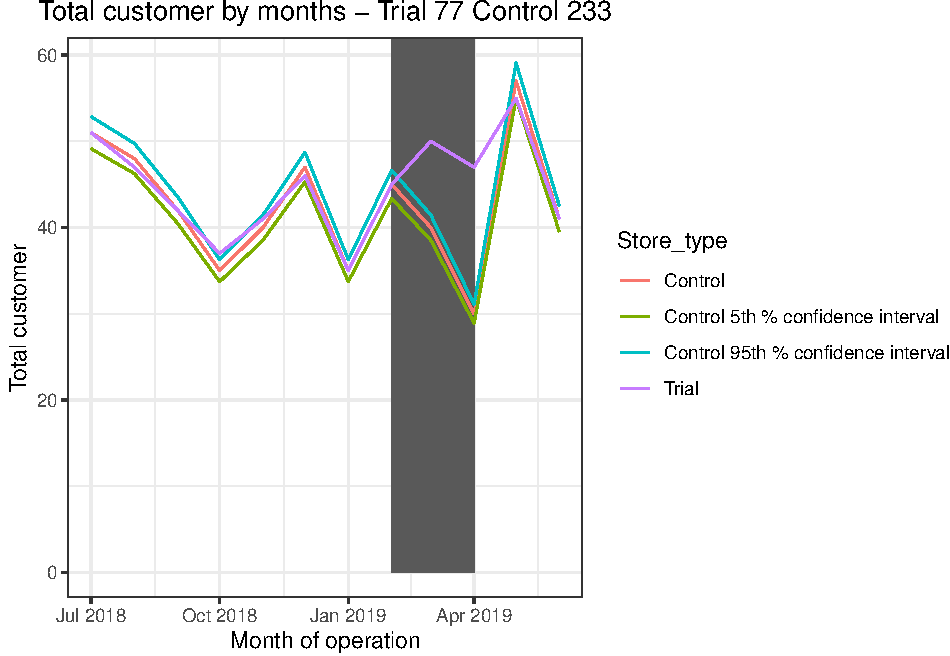
\includegraphics{Untitled_files/figure-latex/unnamed-chunk-7-1} \end{center}

We can see that there is an increase in purchases in December and a
break in late December. Let's zoom in on this.

\begin{Shaded}
\begin{Highlighting}[]
\CommentTok{#### Filter to December and look at individual days}
\CommentTok{# Over to you - recreate the chart above zoomed in to the relevant dates.}
\KeywordTok{ggplot}\NormalTok{(transactions_by_day, }\KeywordTok{aes}\NormalTok{(}\DataTypeTok{x =}\NormalTok{ DATE, }\DataTypeTok{y =}\NormalTok{ N)) }\OperatorTok{+}
\KeywordTok{geom_line}\NormalTok{() }\OperatorTok{+}
\KeywordTok{facet_zoom}\NormalTok{(}\DataTypeTok{x=}\NormalTok{ (DATE}\OperatorTok{>}\KeywordTok{as.Date}\NormalTok{(}\StringTok{'2018-12-01'}\NormalTok{) }\OperatorTok{&}\StringTok{ }\NormalTok{DATE}\OperatorTok{<}\KeywordTok{as.Date}\NormalTok{(}\StringTok{'2019-01-01'}\NormalTok{))) }\OperatorTok{+}
\KeywordTok{labs}\NormalTok{(}\DataTypeTok{x =} \StringTok{"Day"}\NormalTok{, }\DataTypeTok{y =} \StringTok{"Number of transactions"}\NormalTok{, }\DataTypeTok{title =} \StringTok{"Transactions over time"}\NormalTok{) }\OperatorTok{+}
\CommentTok{# scale_x_date(breaks = "1 month") +}
\KeywordTok{theme}\NormalTok{(}\DataTypeTok{axis.text.x =} \KeywordTok{element_text}\NormalTok{(}\DataTypeTok{angle =} \DecValTok{90}\NormalTok{, }\DataTypeTok{vjust =} \FloatTok{0.5}\NormalTok{))}
\end{Highlighting}
\end{Shaded}

\begin{center}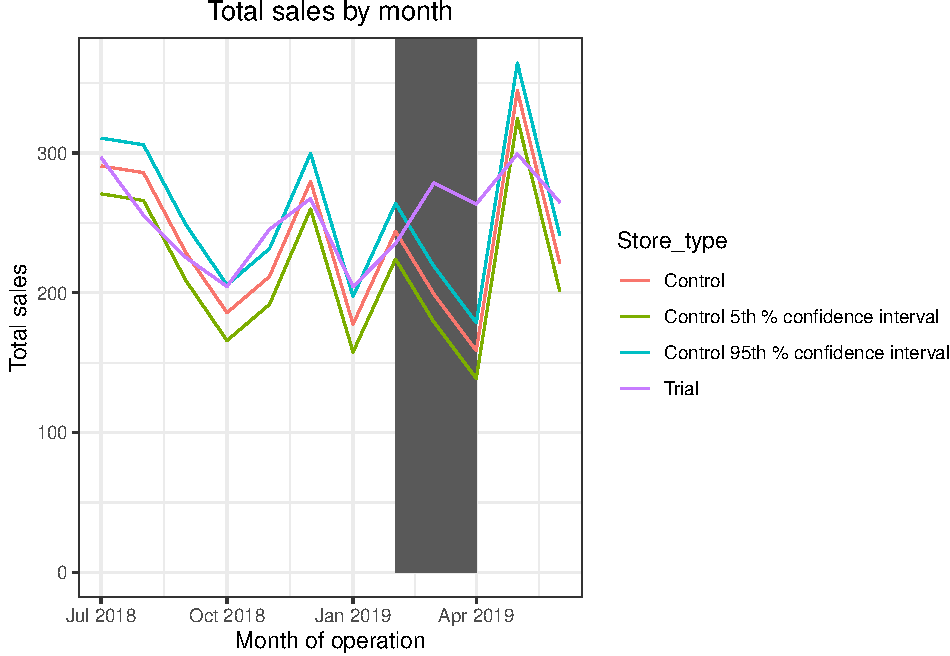
\includegraphics{Untitled_files/figure-latex/unnamed-chunk-8-1} \end{center}

We can see that the increase in sales occurs in the lead-up to Christmas
and that there are zero sales on Christmas day itself. This is due to
shops being closed on Christmas day. Now that we are satisfied that the
data no longer has outliers, we can move on to creating other features
such as brand of chips or pack size from PROD\_NAME. We will start with
pack size.

\begin{Shaded}
\begin{Highlighting}[]
\CommentTok{#### Pack size}
\CommentTok{#### We can work this out by taking the digits that are in PROD_NAME}
\NormalTok{transactionData[, PACK_SIZE }\OperatorTok{:}\ErrorTok{=}\StringTok{ }\KeywordTok{parse_number}\NormalTok{(PROD_NAME)]}
\CommentTok{#### Always check your output}
\CommentTok{#### Let's check if the pack sizes look sensible}
\NormalTok{transactionData[, .N, PACK_SIZE][}\KeywordTok{order}\NormalTok{(PACK_SIZE)]}
\end{Highlighting}
\end{Shaded}

\begin{verbatim}
##     PACK_SIZE     N
##  1:        70  1507
##  2:        90  3008
##  3:       110 22387
##  4:       125  1454
##  5:       134 25102
##  6:       135  3257
##  7:       150 40203
##  8:       160  2970
##  9:       165 15297
## 10:       170 19983
## 11:       175 66390
## 12:       180  1468
## 13:       190  2995
## 14:       200  4473
## 15:       210  6272
## 16:       220  1564
## 17:       250  3169
## 18:       270  6285
## 19:       330 12540
## 20:       380  6416
\end{verbatim}

The largest size is 380g and the smallest size is 70g - seems sensible!

\begin{Shaded}
\begin{Highlighting}[]
\CommentTok{#### Let's plot a histogram of PACK_SIZE since we know that it is a categorical variable and not a continuous variable even though it is numeric.}
\CommentTok{# Over to you! Plot a histogram showing the number of transactions by pack size.}
\KeywordTok{ggplot}\NormalTok{(transactionData, }\KeywordTok{aes}\NormalTok{(}\DataTypeTok{x=}\NormalTok{PACK_SIZE)) }\OperatorTok{+}
\StringTok{  }\KeywordTok{geom_histogram}\NormalTok{(}\DataTypeTok{color =} \StringTok{'darkblue'}\NormalTok{, }\DataTypeTok{fill =} \StringTok{'lightblue'}\NormalTok{, }\DataTypeTok{bins =} \DecValTok{20}\NormalTok{)}
\end{Highlighting}
\end{Shaded}

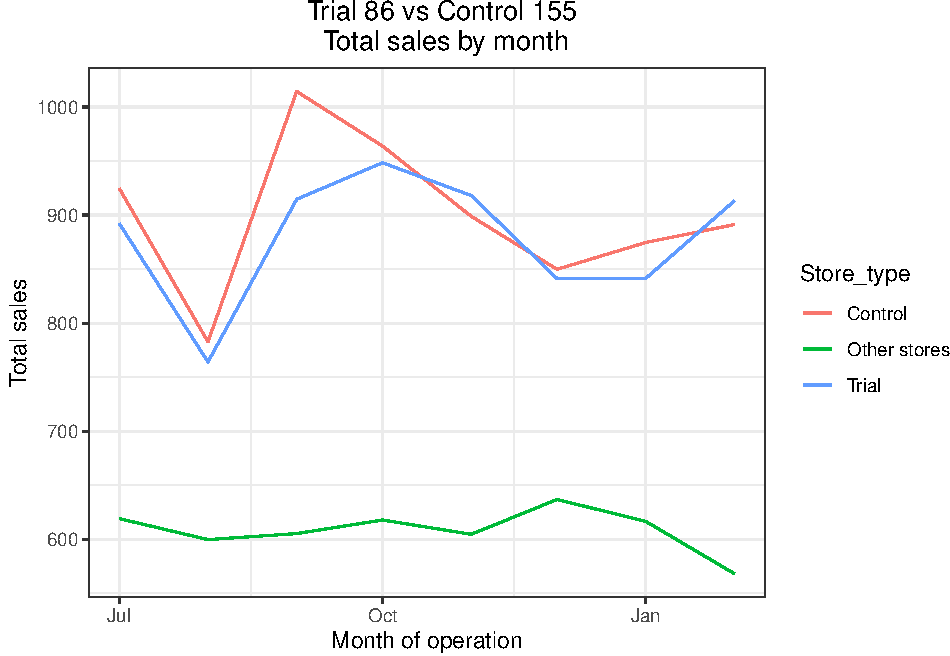
\includegraphics{Untitled_files/figure-latex/unnamed-chunk-9-1.pdf} Pack
sizes created look reasonable. Now to create brands, we can use the
first word in PROD\_NAME to work out the brand name\ldots{}

\begin{Shaded}
\begin{Highlighting}[]
\CommentTok{#### Brands}
\CommentTok{# Over to you! Create a column which contains the brand of the product, by extracting it from the product name.}
\CommentTok{#### Checking brands}
\CommentTok{# Over to you! Check the results look reasonable.}

\NormalTok{transactionData[, BRAND}\OperatorTok{:}\ErrorTok{=}\StringTok{ }\KeywordTok{unlist}\NormalTok{(}\KeywordTok{map}\NormalTok{(}\KeywordTok{strsplit}\NormalTok{(}\KeywordTok{toupper}\NormalTok{(transactionData}\OperatorTok{$}\NormalTok{PROD_NAME), }\StringTok{' '}\NormalTok{),}\DecValTok{1}\NormalTok{))]}
\end{Highlighting}
\end{Shaded}

Some of the brand names look like they are of the same brands - such as
RED and RRD, which are both Red Rock Deli chips. Let's combine these
together.

\begin{Shaded}
\begin{Highlighting}[]
\CommentTok{#### Clean brand names}
\NormalTok{transactionData[BRAND }\OperatorTok{==}\StringTok{ "RED"}\NormalTok{, BRAND }\OperatorTok{:}\ErrorTok{=}\StringTok{ "RRD"}\NormalTok{]}

\CommentTok{# Over to you! Add any additional brand adjustments you think may be required.}
\NormalTok{transactionData[BRAND }\OperatorTok{==}\StringTok{ "NATURAL"}\NormalTok{, BRAND }\OperatorTok{:}\ErrorTok{=}\StringTok{ "NCC"}\NormalTok{]}
\NormalTok{transactionData[BRAND }\OperatorTok{==}\StringTok{ "SMITH"}\NormalTok{, BRAND }\OperatorTok{:}\ErrorTok{=}\StringTok{ "SMITHS"}\NormalTok{]}
\NormalTok{transactionData[BRAND }\OperatorTok{==}\StringTok{ "GRAIN"}\NormalTok{, BRAND }\OperatorTok{:}\ErrorTok{=}\StringTok{ "GRNWVES"}\NormalTok{]}
\NormalTok{transactionData[BRAND }\OperatorTok{==}\StringTok{ "SUNBITES"}\NormalTok{, BRAND }\OperatorTok{:}\ErrorTok{=}\StringTok{ "SNBTS"}\NormalTok{]}
\NormalTok{transactionData[BRAND }\OperatorTok{==}\StringTok{ "INFUZIONS"}\NormalTok{, BRAND }\OperatorTok{:}\ErrorTok{=}\StringTok{ "INFZNS"}\NormalTok{]}
\NormalTok{transactionData[BRAND }\OperatorTok{==}\StringTok{ "DORITO"}\NormalTok{, BRAND }\OperatorTok{:}\ErrorTok{=}\StringTok{ "DORITOS"}\NormalTok{]}

\CommentTok{#### Check again}
\CommentTok{# Over to you! Check the results look reasonable.}
\NormalTok{transactionData[, .N, BRAND][}\KeywordTok{order}\NormalTok{(}\OperatorTok{-}\NormalTok{N)]}
\end{Highlighting}
\end{Shaded}

\begin{verbatim}
##          BRAND     N
##  1:     KETTLE 41288
##  2:     SMITHS 30353
##  3:    DORITOS 25224
##  4:   PRINGLES 25102
##  5:        RRD 16321
##  6:     INFZNS 14201
##  7:      THINS 14075
##  8:         WW 10320
##  9:       COBS  9693
## 10:   TOSTITOS  9471
## 11:   TWISTIES  9454
## 12:    GRNWVES  7740
## 13:        NCC  7469
## 14:   TYRRELLS  6442
## 15:   CHEEZELS  4603
## 16:        CCS  4551
## 17:      SNBTS  3008
## 18:    CHEETOS  2927
## 19:     BURGER  1564
## 20: WOOLWORTHS  1516
## 21:     FRENCH  1418
##          BRAND     N
\end{verbatim}

\hypertarget{examining-customer-data}{%
\subsubsection{Examining customer data}\label{examining-customer-data}}

Now that we are happy with the transaction dataset, let's have a look at
the customer dataset.

\begin{Shaded}
\begin{Highlighting}[]
\CommentTok{#### Examining customer data}
\CommentTok{# Over to you! Do some basic summaries of the dataset, including distributions of any key columns.}
\KeywordTok{str}\NormalTok{(customerData)}
\end{Highlighting}
\end{Shaded}

\begin{verbatim}
## Classes 'data.table' and 'data.frame': 72637 obs. of 3 variables:
## $ LYLTY_CARD_NBR : int 1000 1002 1003 1004 1005 1007 1009 1010 1011 1012 ...
## $ LIFESTAGE : chr "YOUNG SINGLES/COUPLES" "YOUNG SINGLES/COUPLES" "YOUNG
FAMILIES" "OLDER SINGLES/COUPLES" ...
## $ PREMIUM_CUSTOMER: chr "Premium" "Mainstream" "Budget" "Mainstream" ...
## - attr(*, ".internal.selfref")=<externalptr>
\end{verbatim}

\begin{Shaded}
\begin{Highlighting}[]
\NormalTok{customerData[, .N, LIFESTAGE][}\KeywordTok{order}\NormalTok{(}\OperatorTok{-}\NormalTok{N)]}
\end{Highlighting}
\end{Shaded}

\begin{verbatim}
##                 LIFESTAGE     N
## 1:               RETIREES 14805
## 2:  OLDER SINGLES/COUPLES 14609
## 3:  YOUNG SINGLES/COUPLES 14441
## 4:         OLDER FAMILIES  9780
## 5:         YOUNG FAMILIES  9178
## 6: MIDAGE SINGLES/COUPLES  7275
## 7:           NEW FAMILIES  2549
\end{verbatim}

\begin{Shaded}
\begin{Highlighting}[]
\NormalTok{customerData[, .N, PREMIUM_CUSTOMER][}\KeywordTok{order}\NormalTok{(}\OperatorTok{-}\NormalTok{N)]}
\end{Highlighting}
\end{Shaded}

\begin{verbatim}
##    PREMIUM_CUSTOMER     N
## 1:       Mainstream 29245
## 2:           Budget 24470
## 3:          Premium 18922
\end{verbatim}

\begin{Shaded}
\begin{Highlighting}[]
\CommentTok{#### Merge transaction data to customer data}
\NormalTok{data <-}\StringTok{ }\KeywordTok{merge}\NormalTok{(transactionData, customerData, }\DataTypeTok{all.x =} \OtherTok{TRUE}\NormalTok{)}
\end{Highlighting}
\end{Shaded}

As the number of rows in \texttt{data} is the same as that of
\texttt{transactionData}, we can be sure that no duplicates were
created. This is because we created \texttt{data} by setting
\texttt{all.x\ =\ TRUE} (in other words, a left join) which means take
all the rows in \texttt{transactionData} and find rows with matching
values in shared columns and then joining the details in these rows to
the \texttt{x} or the first mentioned table.

Let's also check if some customers were not matched on by checking for
nulls.

\begin{Shaded}
\begin{Highlighting}[]
\CommentTok{# Over to you! See if any transactions did not have a matched customer.}
\NormalTok{data[}\KeywordTok{is.null}\NormalTok{(LIFESTAGE), .N]}
\end{Highlighting}
\end{Shaded}

\begin{verbatim}
## [1] 0
\end{verbatim}

\begin{Shaded}
\begin{Highlighting}[]
\NormalTok{data[}\KeywordTok{is.null}\NormalTok{(PREMIUM_CUSTOMER), .N]}
\end{Highlighting}
\end{Shaded}

\begin{verbatim}
## [1] 0
\end{verbatim}

Great, there are no nulls! So all our customers in the transaction data
has been accounted for in the customer dataset.\\
Note that if you are continuing with Task 2, you may want to retain this
dataset which you can write out as a csv.

\begin{Shaded}
\begin{Highlighting}[]
\KeywordTok{fwrite}\NormalTok{(data, }\KeywordTok{paste0}\NormalTok{(filePath,}\StringTok{"QVI_data.csv"}\NormalTok{))}
\end{Highlighting}
\end{Shaded}

Data exploration is now complete!

\hypertarget{data-analysis-on-customer-segments}{%
\subsection{Data analysis on customer
segments}\label{data-analysis-on-customer-segments}}

Now that the data is ready for analysis, we can define some metrics of
interest to the client:

\begin{itemize}
\item
  Who spends the most on chips (total sales), describing customers by
  lifestage and how premium their general purchasing behaviour is

  \begin{itemize}
  \tightlist
  \item
    How many customers are in each segment
  \item
    How many chips are bought per customer by segment
  \item
    What's the average chip price by customer segment
  \end{itemize}
\item
  We could also ask our data team for more information. Examples are:

  \begin{itemize}
  \tightlist
  \item
    The customer's total spend over the period and total spend for each
    transaction to understand what proportion of their grocery spend is
    on chip
  \item
    Proportion of customers in each customer segment overall to compare
    against the mix of customers who purchase chips
  \end{itemize}
\end{itemize}

Let's start with calculating total sales by LIFESTAGE and
PREMIUM\_CUSTOMER and plotting the split by these segments to describe
which customer segment contribute most to chip sales.

\begin{Shaded}
\begin{Highlighting}[]
\CommentTok{#### Total sales by LIFESTAGE and PREMIUM_CUSTOMER}
\CommentTok{# Over to you! Calculate the summary of sales by those dimensions and create a plot.}

\CommentTok{# sales <- data %>%}
\CommentTok{#   group_by(LIFESTAGE, PREMIUM_CUSTOMER) %>%}
\CommentTok{#   summarise(SALES = sum(TOT_SALES))}
\NormalTok{sales <-}\StringTok{ }\NormalTok{data[, .(}\DataTypeTok{SALES =} \KeywordTok{sum}\NormalTok{(TOT_SALES)), .(LIFESTAGE, PREMIUM_CUSTOMER)]}
\NormalTok{p <-}\StringTok{ }\KeywordTok{ggplot}\NormalTok{(}\DataTypeTok{data =}\NormalTok{ sales) }\OperatorTok{+}
\StringTok{  }\KeywordTok{geom_mosaic}\NormalTok{(}\KeywordTok{aes}\NormalTok{(}\DataTypeTok{weight =}\NormalTok{ SALES, }\DataTypeTok{x =} \KeywordTok{product}\NormalTok{(PREMIUM_CUSTOMER, LIFESTAGE),}
                  \DataTypeTok{fill =}\NormalTok{ PREMIUM_CUSTOMER)) }\OperatorTok{+}
\StringTok{  }\KeywordTok{labs}\NormalTok{(}\DataTypeTok{x =} \StringTok{"Lifestage"}\NormalTok{, }\DataTypeTok{y =} \StringTok{"Premium customer flag"}\NormalTok{, }
       \DataTypeTok{title =} \StringTok{"Proportion of sales"}\NormalTok{) }\OperatorTok{+}
\StringTok{  }\KeywordTok{theme}\NormalTok{(}\DataTypeTok{axis.text.x =} \KeywordTok{element_text}\NormalTok{(}\DataTypeTok{angle =} \DecValTok{90}\NormalTok{, }\DataTypeTok{vjust =} \FloatTok{0.5}\NormalTok{))}
\NormalTok{p}\OperatorTok{+}\StringTok{ }\KeywordTok{geom_text}\NormalTok{(}\DataTypeTok{data =} \KeywordTok{ggplot_build}\NormalTok{(p)}\OperatorTok{$}\NormalTok{data[[}\DecValTok{1}\NormalTok{]], }
             \KeywordTok{aes}\NormalTok{(}\DataTypeTok{x =}\NormalTok{ (xmin}\OperatorTok{+}\NormalTok{xmax)}\OperatorTok{/}\DecValTok{2}\NormalTok{, }\DataTypeTok{y =}\NormalTok{ (ymin}\OperatorTok{+}\NormalTok{ymax)}\OperatorTok{/}\DecValTok{2}\NormalTok{, }
              \DataTypeTok{label =} \KeywordTok{as.character}\NormalTok{(}\KeywordTok{paste}\NormalTok{(}\KeywordTok{round}\NormalTok{(.wt}\OperatorTok{/}\KeywordTok{sum}\NormalTok{(.wt),}\DecValTok{3}\NormalTok{)}\OperatorTok{*}\DecValTok{100}\NormalTok{, }\StringTok{'%'}\NormalTok{))))}
\end{Highlighting}
\end{Shaded}

\begin{verbatim}
## Warning: `unite_()` was deprecated in tidyr 1.2.0.
## Please use `unite()` instead.
## This warning is displayed once every 8 hours.
## Call `lifecycle::last_lifecycle_warnings()` to see where this warning was generated.
\end{verbatim}

\begin{center}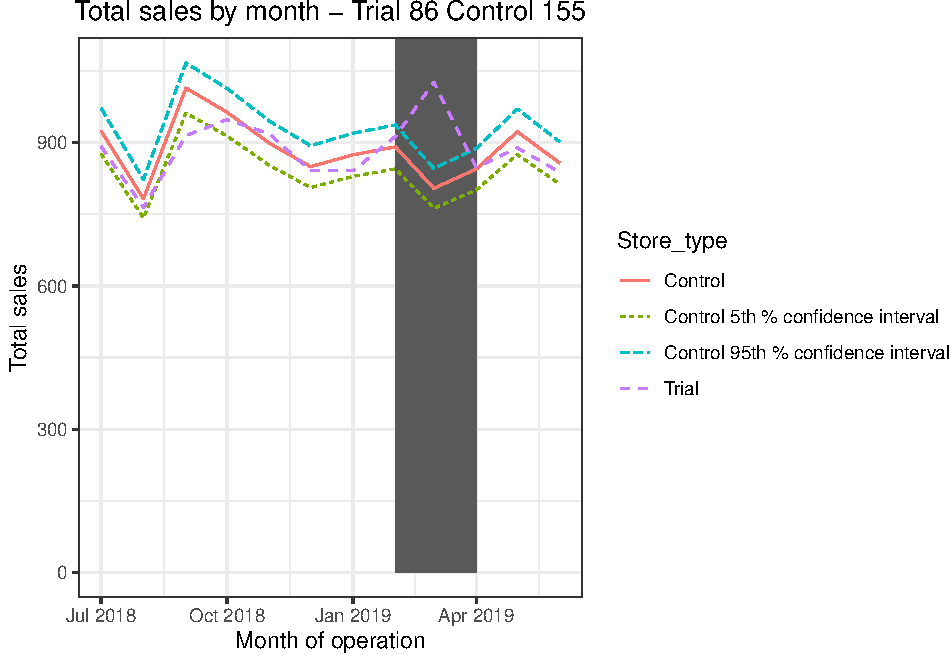
\includegraphics{Untitled_files/figure-latex/unnamed-chunk-11-1} \end{center}

Sales are coming mainly from Budget - older families, Mainstream - young
singles/couples, and Mainstream - retirees\\
Let's see if the higher sales are due to there being more customers who
buy chips.

\begin{Shaded}
\begin{Highlighting}[]
\CommentTok{#### Number of customers by LIFESTAGE and PREMIUM_CUSTOMER}
\CommentTok{# Over to you! Calculate the summary of number of customers by those dimensions and create a plot.}
\NormalTok{n_cust <-}\StringTok{ }\NormalTok{data[, .(}\DataTypeTok{N_CUST =} \KeywordTok{uniqueN}\NormalTok{(LYLTY_CARD_NBR)), }
\NormalTok{               .(LIFESTAGE, PREMIUM_CUSTOMER)][}\KeywordTok{order}\NormalTok{(}\OperatorTok{-}\NormalTok{N_CUST)]}
\CommentTok{#### create plot}
\NormalTok{p <-}\StringTok{ }\KeywordTok{ggplot}\NormalTok{(}\DataTypeTok{data =}\NormalTok{ n_cust) }\OperatorTok{+}
\StringTok{  }\KeywordTok{geom_mosaic}\NormalTok{(}\KeywordTok{aes}\NormalTok{(}\DataTypeTok{weight =}\NormalTok{ N_CUST, }
                  \DataTypeTok{x =} \KeywordTok{product}\NormalTok{(PREMIUM_CUSTOMER, LIFESTAGE),}
                  \DataTypeTok{fill =}\NormalTok{ PREMIUM_CUSTOMER)) }\OperatorTok{+}
\StringTok{  }\KeywordTok{labs}\NormalTok{(}\DataTypeTok{x =} \StringTok{"Lifestage"}\NormalTok{, }\DataTypeTok{y =} \StringTok{"Premium customer flag"}\NormalTok{,}
       \DataTypeTok{title =} \StringTok{'Proportion of customers'}\NormalTok{) }\OperatorTok{+}
\StringTok{  }\KeywordTok{theme}\NormalTok{(}\DataTypeTok{axis.text.x =} \KeywordTok{element_text}\NormalTok{(}\DataTypeTok{angle =} \DecValTok{90}\NormalTok{, }\DataTypeTok{vjust =} \FloatTok{0.5}\NormalTok{))}
\NormalTok{p }\OperatorTok{+}\StringTok{ }\KeywordTok{geom_text}\NormalTok{(}\DataTypeTok{data =} \KeywordTok{ggplot_build}\NormalTok{(p)}\OperatorTok{$}\NormalTok{data[[}\DecValTok{1}\NormalTok{]],}
              \KeywordTok{aes}\NormalTok{(}\DataTypeTok{x =}\NormalTok{(xmin}\OperatorTok{+}\NormalTok{xmax)}\OperatorTok{/}\DecValTok{2}\NormalTok{, }\DataTypeTok{y =}\NormalTok{ (ymin}\OperatorTok{+}\NormalTok{ymax)}\OperatorTok{/}\DecValTok{2}\NormalTok{,}
                  \DataTypeTok{label =} \KeywordTok{as.character}\NormalTok{(}\KeywordTok{paste}\NormalTok{(}\KeywordTok{round}\NormalTok{(.wt}\OperatorTok{/}\KeywordTok{sum}\NormalTok{(.wt),}\DecValTok{3}\NormalTok{)}\OperatorTok{*}\DecValTok{100}\NormalTok{, }\StringTok{'%'}\NormalTok{)))}
\NormalTok{              )}
\end{Highlighting}
\end{Shaded}

\begin{center}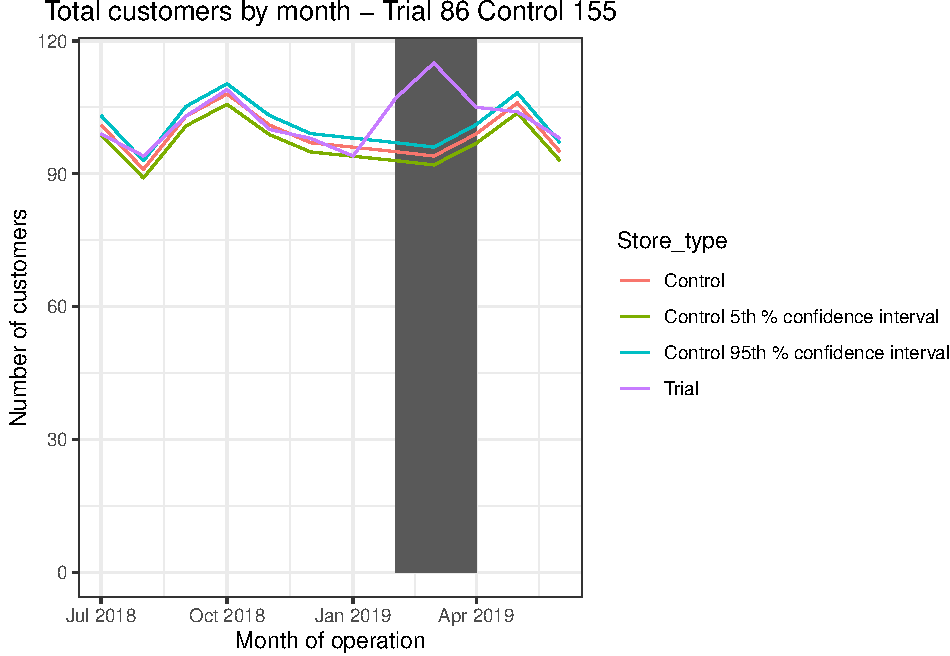
\includegraphics{Untitled_files/figure-latex/unnamed-chunk-12-1} \end{center}

There are more Mainstream - young singles/couples and Mainstream -
retirees who buy chips. This con- tributes to there being more sales to
these customer segments but this is not a major driver for the Budget -
Older families segment.

Higher sales may also be driven by more units of chips being bought per
customer. Let's have a look at this next.

\begin{Shaded}
\begin{Highlighting}[]
\CommentTok{#### Average number of units per customer by LIFESTAGE and PREMIUM_CUSTOMER}
\CommentTok{# Over to you! Calculate and plot the average number of units per customer by those two dimensions.}
\NormalTok{avg_units <-}\StringTok{ }\NormalTok{data[, .(}\DataTypeTok{AVG_UNITS =} \KeywordTok{sum}\NormalTok{(PROD_QTY)}\OperatorTok{/}\KeywordTok{uniqueN}\NormalTok{(LYLTY_CARD_NBR)),}
\NormalTok{                  .(LIFESTAGE, PREMIUM_CUSTOMER)][}\KeywordTok{order}\NormalTok{(}\OperatorTok{-}\NormalTok{AVG_UNITS)]}
\KeywordTok{ggplot}\NormalTok{(}\DataTypeTok{data =}\NormalTok{ avg_units, }
            \KeywordTok{aes}\NormalTok{(}\DataTypeTok{weight =}\NormalTok{ AVG_UNITS, }\DataTypeTok{x =}\NormalTok{ LIFESTAGE, }\DataTypeTok{fill =}\NormalTok{ PREMIUM_CUSTOMER)) }\OperatorTok{+}
\StringTok{  }\KeywordTok{geom_bar}\NormalTok{(}\DataTypeTok{position =} \KeywordTok{position_dodge}\NormalTok{())}\OperatorTok{+}
\StringTok{  }\KeywordTok{labs}\NormalTok{(}\DataTypeTok{x =} \StringTok{'Lifestage'}\NormalTok{, }\DataTypeTok{y =} \StringTok{'Avg units per transaction'}\NormalTok{, }
       \DataTypeTok{title =} \StringTok{'Units per customer'}\NormalTok{) }\OperatorTok{+}
\StringTok{  }\KeywordTok{theme}\NormalTok{(}\DataTypeTok{axis.text.x =} \KeywordTok{element_text}\NormalTok{(}\DataTypeTok{angle =} \DecValTok{90}\NormalTok{, }\DataTypeTok{vjust =} \FloatTok{0.5}\NormalTok{))}
\end{Highlighting}
\end{Shaded}

\begin{center}\includegraphics{Untitled_files/figure-latex/unnamed-chunk-13-1} \end{center}

Older families and young families in general buy more chips per
customer.

Let's also investigate the average price per unit chips bought for each
customer segment as this is also a driver of total sales.

\begin{Shaded}
\begin{Highlighting}[]
\CommentTok{#### Average price per unit by LIFESTAGE and PREMIUM_CUSTOMER}
\CommentTok{# Over to you! Calculate and plot the average price per unit sold (average sale price) by those two customer dimensions.}
\NormalTok{unit_price <-}\StringTok{ }\NormalTok{data[, .(}\DataTypeTok{UNIT_PRICE =} \KeywordTok{sum}\NormalTok{(TOT_SALES)}\OperatorTok{/}\KeywordTok{sum}\NormalTok{(PROD_QTY)),}
\NormalTok{                   .(LIFESTAGE, PREMIUM_CUSTOMER)][}\KeywordTok{order}\NormalTok{(}\OperatorTok{-}\NormalTok{UNIT_PRICE)]}
\KeywordTok{ggplot}\NormalTok{(}\DataTypeTok{data =}\NormalTok{ unit_price, }
       \KeywordTok{aes}\NormalTok{(}\DataTypeTok{weight =}\NormalTok{ UNIT_PRICE, }\DataTypeTok{x =}\NormalTok{ LIFESTAGE, }\DataTypeTok{fill =}\NormalTok{ PREMIUM_CUSTOMER)) }\OperatorTok{+}
\StringTok{  }\KeywordTok{geom_bar}\NormalTok{(}\DataTypeTok{position =} \KeywordTok{position_dodge}\NormalTok{()) }\OperatorTok{+}
\StringTok{  }\KeywordTok{labs}\NormalTok{(}\DataTypeTok{x =} \StringTok{'Lifestage'}\NormalTok{, }\DataTypeTok{y =} \StringTok{'Avg price per units'}\NormalTok{, }
       \DataTypeTok{title =} \StringTok{'Price per units'}\NormalTok{) }\OperatorTok{+}
\StringTok{  }\KeywordTok{theme}\NormalTok{(}\DataTypeTok{axis.text.x =} \KeywordTok{element_text}\NormalTok{(}\DataTypeTok{angle =} \DecValTok{90}\NormalTok{, }\DataTypeTok{vjust =} \FloatTok{0.5}\NormalTok{))}
\end{Highlighting}
\end{Shaded}

\begin{center}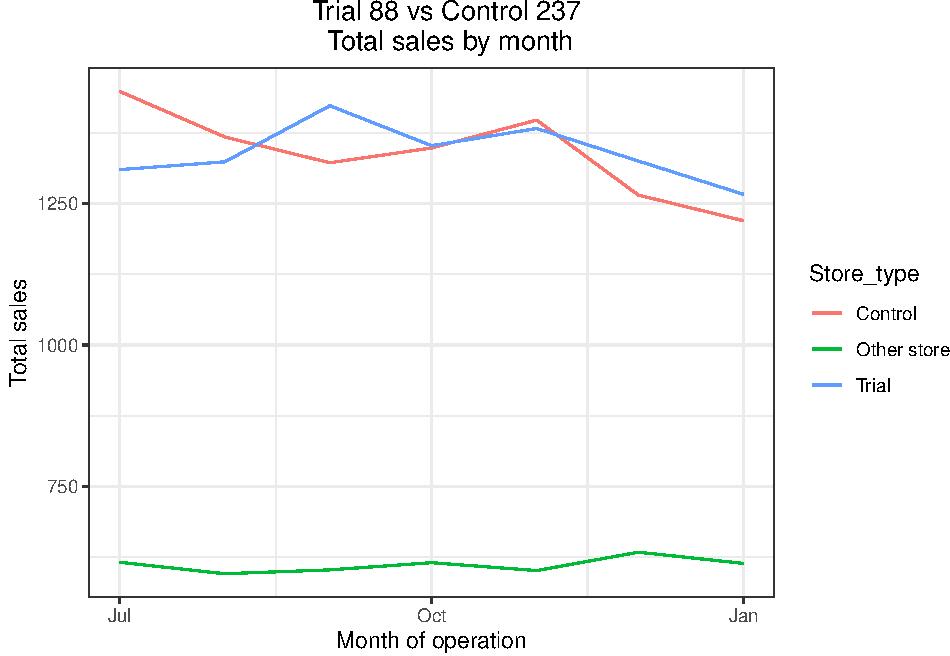
\includegraphics{Untitled_files/figure-latex/unnamed-chunk-14-1} \end{center}

Mainstream midage and young singles and couples are more willing to pay
more per packet of chips compared to their budget and premium
counterparts. This may be due to premium shoppers being more likely to
buy healthy snacks and when they buy chips, this is mainly for
entertainment purposes rather than their own consumption. This is also
supported by there being fewer premium midage and young singles and
couples buying chips compared to their mainstream counterparts.

As the difference in average price per unit isn't large, we can check if
this difference is statistically different.

\begin{Shaded}
\begin{Highlighting}[]
\CommentTok{#### Perform an independent t-test between mainstream vs premium and budget midage and}
\CommentTok{#### young singles and couples}
\CommentTok{# Over to you! Perform a t-test to see if the difference is significant.}
\NormalTok{data[, UNIT_PRICE}\OperatorTok{:}\ErrorTok{=}\StringTok{ }\NormalTok{TOT_SALES}\OperatorTok{/}\NormalTok{PROD_QTY]}
\KeywordTok{t.test}\NormalTok{(data[PREMIUM_CUSTOMER}\OperatorTok{==}\StringTok{'Mainstream'} \OperatorTok{&}\StringTok{ }
\StringTok{                  }\NormalTok{LIFESTAGE }\OperatorTok\StringTok{ }\KeywordTok{c}\NormalTok{(}\StringTok{'YOUNG SINGLES/COUPLES'}\NormalTok{, }\StringTok{'MIDAGE SINGLES/COUPLES'}\NormalTok{), UNIT_PRICE], }
\NormalTok{       data[PREMIUM_CUSTOMER}\OperatorTok{!=}\StringTok{'Mainstream'} \OperatorTok{&}\StringTok{ }
\StringTok{                  }\NormalTok{LIFESTAGE }\OperatorTok\StringTok{ }\KeywordTok{c}\NormalTok{(}\StringTok{'YOUNG SINGLES/COUPLES'}\NormalTok{, }\StringTok{'MIDAGE SINGLES/COUPLES'}\NormalTok{), UNIT_PRICE],}
       \DataTypeTok{alternative =} \StringTok{'greater'}\NormalTok{)}
\end{Highlighting}
\end{Shaded}

\begin{verbatim}
##
## Welch Two Sample t-test
##
## data: data[PREMIUM_CUSTOMER == "Mainstream" & LIFESTAGE %in% c("YOUNG
SINGLES/COUPLES", "MIDAGE SINGLES/COUPLES"), UNIT_PRICE] and
data[PREMIUM_CUSTOMER != "Mainstream" & LIFESTAGE %in% c("YOUNG
SINGLES/COUPLES", "MIDAGE SINGLES/COUPLES"), UNIT_PRICE]
## t = 37.624, df = 54791, p-value < 2.2e-16
## alternative hypothesis: true difference in means is greater than 0
## 95 percent confidence interval:
## 0.3187234 Inf
## sample estimates:
## mean of x mean of y
## 4.039786 3.706491
\end{verbatim}

\begin{Shaded}
\begin{Highlighting}[]
\NormalTok{data <-}\StringTok{ }\KeywordTok{subset}\NormalTok{(data, }\DataTypeTok{select =} \OperatorTok{-}\NormalTok{UNIT_PRICE)}
\end{Highlighting}
\end{Shaded}

The t-test results in a p-value \textless{} 2.2e-16, i.e.~the unit price
for mainstream, young and mid-age singles and couples are significantly
higher than that of budget or premium, young and midage singles and
couples.

\hypertarget{deep-dive-into-specific-customer-segments-for-insights}{%
\subsection{Deep dive into specific customer segments for
insights}\label{deep-dive-into-specific-customer-segments-for-insights}}

We have found quite a few interesting insights that we can dive deeper
into.

We might want to target customer segments that contribute the most to
sales to retain them or further increase sales. Let's look at Mainstream
- young singles/couples. For instance, let's find out if they tend to
buy a particular brand of chips.

\begin{Shaded}
\begin{Highlighting}[]
\CommentTok{#### Deep dive into Mainstream, young singles/couples}
\CommentTok{# Over to you! Work out of there are brands that these two customer segments prefer more than others. You could use a technique called affinity analysis or a-priori analysis (or any other method if you prefer)}
\NormalTok{segment1 <-}\StringTok{ }\NormalTok{data[PREMIUM_CUSTOMER }\OperatorTok{==}\StringTok{'Mainstream'}\OperatorTok{&}
\StringTok{                 }\NormalTok{LIFESTAGE }\OperatorTok{==}\StringTok{'YOUNG SINGLES/COUPLES'}\NormalTok{, ]}
\NormalTok{other <-}\StringTok{ }\NormalTok{data[}\OperatorTok{!}\NormalTok{(PREMIUM_CUSTOMER }\OperatorTok{==}\StringTok{'Mainstream'}\OperatorTok{&}
\StringTok{                 }\NormalTok{LIFESTAGE }\OperatorTok{==}\StringTok{'YOUNG SINGLES/COUPLES'}\NormalTok{), ]}
\CommentTok{# Brand affinity compared to the rest of the population}
\NormalTok{qty_segment1 <-}\StringTok{ }\NormalTok{segment1[, }\KeywordTok{sum}\NormalTok{(PROD_QTY)]}
\NormalTok{qty_other <-}\StringTok{ }\NormalTok{other[, }\KeywordTok{sum}\NormalTok{(PROD_QTY)]}
\NormalTok{brand_qty_segment1 <-}\StringTok{ }\NormalTok{segment1[, .(}\DataTypeTok{targetSegment =} \KeywordTok{sum}\NormalTok{(PROD_QTY)}\OperatorTok{/}\NormalTok{qty_segment1),}
\NormalTok{                              by =}\StringTok{ }\NormalTok{BRAND]}
\NormalTok{brand_qty_other <-}\StringTok{ }\NormalTok{other[, .(}\DataTypeTok{other =} \KeywordTok{sum}\NormalTok{(PROD_QTY)}\OperatorTok{/}\NormalTok{qty_other),}
\NormalTok{                         by =}\StringTok{ }\NormalTok{BRAND]}
\NormalTok{brand_proportions <-}\StringTok{ }\KeywordTok{merge}\NormalTok{(brand_qty_segment1, }
\NormalTok{                           brand_qty_other)[, affinityToBrand }\OperatorTok{:}\ErrorTok{=}\StringTok{ }\NormalTok{targetSegment}\OperatorTok{/}\NormalTok{other]}
\NormalTok{brand_proportions[}\KeywordTok{order}\NormalTok{(}\OperatorTok{-}\NormalTok{affinityToBrand)]}
\end{Highlighting}
\end{Shaded}

\begin{verbatim}
##          BRAND targetSegment       other affinityToBrand
##  1:   TYRRELLS   0.031552795 0.025692464       1.2280953
##  2:   TWISTIES   0.046183575 0.037876520       1.2193194
##  3:    DORITOS   0.122760524 0.101074684       1.2145526
##  4:     KETTLE   0.197984817 0.165553442       1.1958967
##  5:   TOSTITOS   0.045410628 0.037977861       1.1957131
##  6:   PRINGLES   0.119420290 0.100634769       1.1866703
##  7:       COBS   0.044637681 0.039048861       1.1431238
##  8:     INFZNS   0.064679089 0.057064679       1.1334347
##  9:      THINS   0.060372671 0.056986370       1.0594230
## 10:    GRNWVES   0.032712215 0.031187957       1.0488733
## 11:   CHEEZELS   0.017971014 0.018646902       0.9637534
## 12:     SMITHS   0.096369910 0.124583692       0.7735355
## 13:     FRENCH   0.003947550 0.005758060       0.6855694
## 14:    CHEETOS   0.008033126 0.012066591       0.6657329
## 15:        RRD   0.043809524 0.067493678       0.6490908
## 16:        NCC   0.019599724 0.030853989       0.6352412
## 17:        CCS   0.011180124 0.018895650       0.5916771
## 18:      SNBTS   0.006349206 0.012580210       0.5046980
## 19:         WW   0.021256039 0.043049561       0.4937574
## 20: WOOLWORTHS   0.002843340 0.006377627       0.4458304
## 21:     BURGER   0.002926156 0.006596434       0.4435967
##          BRAND targetSegment       other affinityToBrand
\end{verbatim}

We can see that :

\begin{itemize}
\tightlist
\item
  Mainstream young singles/couples are 23\% more likely to purchase
  Tyrrells chips compared to the rest of the population
\item
  Mainstreamyoungsingles/couplesare56\%lesslikelytopurchaseBurgerRingscomparedtotherest
  of the population
\end{itemize}

Let's also find out if our target segment tends to buy larger packs of
chips.

\begin{Shaded}
\begin{Highlighting}[]
\CommentTok{#### Preferred pack size compared to the rest of the population}
\CommentTok{# Over to you! Do the same for pack size.}
\NormalTok{qty_segment1_by_packSize <-}\StringTok{ }\NormalTok{segment1[, .(}\DataTypeTok{targetSegment =} \KeywordTok{sum}\NormalTok{(PROD_QTY)}\OperatorTok{/}\NormalTok{qty_segment1),}
\NormalTok{                              by =}\StringTok{ }\NormalTok{PACK_SIZE]}
\NormalTok{qty_other_by_packSize <-}\StringTok{ }\NormalTok{other[, .(}\DataTypeTok{other =} \KeywordTok{sum}\NormalTok{(PROD_QTY)}\OperatorTok{/}\NormalTok{qty_other),}
\NormalTok{                         by =}\StringTok{ }\NormalTok{PACK_SIZE]}
\NormalTok{packSize_proportions <-}\StringTok{ }\KeywordTok{merge}\NormalTok{(qty_segment1_by_packSize, }
\NormalTok{                           qty_other_by_packSize)[, affinityToPackSize }\OperatorTok{:}\ErrorTok{=}\StringTok{ }\NormalTok{targetSegment}\OperatorTok{/}\NormalTok{other]}
\NormalTok{packSize_proportions[}\KeywordTok{order}\NormalTok{(}\OperatorTok{-}\NormalTok{affinityToPackSize)]}
\end{Highlighting}
\end{Shaded}

\begin{verbatim}
##     PACK_SIZE targetSegment       other affinityToPackSize
##  1:       270   0.031828847 0.025095929          1.2682873
##  2:       380   0.032160110 0.025584213          1.2570295
##  3:       330   0.061283644 0.050161917          1.2217166
##  4:       134   0.119420290 0.100634769          1.1866703
##  5:       110   0.106280193 0.089791190          1.1836372
##  6:       210   0.029123533 0.025121265          1.1593180
##  7:       135   0.014768806 0.013075403          1.1295106
##  8:       250   0.014354727 0.012780590          1.1231662
##  9:       170   0.080772947 0.080985964          0.9973697
## 10:       150   0.157598344 0.163420656          0.9643722
## 11:       175   0.254989648 0.270006956          0.9443818
## 12:       165   0.055652174 0.062267662          0.8937572
## 13:       190   0.007481021 0.012442016          0.6012708
## 14:       180   0.003588682 0.006066692          0.5915385
## 15:       160   0.006404417 0.012372920          0.5176157
## 16:        90   0.006349206 0.012580210          0.5046980
## 17:       125   0.003008972 0.006036750          0.4984423
## 18:       200   0.008971705 0.018656115          0.4808989
## 19:        70   0.003036577 0.006322350          0.4802924
## 20:       220   0.002926156 0.006596434          0.4435967
\end{verbatim}

It looks like Mainstream young singles/couples are 27\% more likely to
purchase a 270g pack of chips com- pared to the rest of the population
but let's dive into what brands sell this pack size.

\begin{Shaded}
\begin{Highlighting}[]
\NormalTok{data[PACK_SIZE }\OperatorTok{==}\DecValTok{270}\NormalTok{, }\KeywordTok{unique}\NormalTok{(PROD_NAME)]}
\end{Highlighting}
\end{Shaded}

\begin{verbatim}
## [1] "Twisties Cheese     270g" "Twisties Chicken270g"
\end{verbatim}

Twisties are the only brand offering 270g packs and so this may instead
be reflecting a higher likelihood of purchasing Twisties.

\hypertarget{conclusion}{%
\subsection{Conclusion}\label{conclusion}}

Let's recap what we've found!\\
Sales have mainly been due to Budget - older families, Mainstream -
young singles/couples, and Mainstream - retirees shoppers. We found that
the high spend in chips for mainstream young singles/couples and re-
tirees is due to there being more of them than other buyers. Mainstream,
midage and young singles and couples are also more likely to pay more
per packet of chips. This is indicative of impulse buying behaviour.
We've also found that Mainstream young singles and couples are 23\% more
likely to purchase Tyrrells chips compared to the rest of the
population. The Category Manager may want to increase the category's
per- formance by off-locating some Tyrrells and smaller packs of chips
in discretionary space near segments where young singles and couples
frequent more often to increase visibilty and impulse behaviour.

Quantium can help the Category Manager with recommendations of where
these segments are and further help them with measuring the impact of
the changed placement. We'll work on measuring the impact of trials in
the next task and putting all these together in the third task.

\end{document}
